\chapter{Scalability evaluation}
%Block delay attack, Ramsomware attack의 공격과는 달리 DRAIN attack 의 경우는 스마트 컨트랙트상의 취약한 패턴의 로직이 존재 하여야만 공격이 성공 하는 것을 알수 있다. 때문에 이러한 패턴의 스마트 컨트랙트가 얼마나 많이 존재하는지를 확장하여 평가 하기 위해 아래와 같은 scalability를 고려한 evaluation tool을 개발하였다.
The Resource-drain-attacks are supposed to have patterns of vulnerabilities unlike Block delay attack, and Ramsomware attack. Thus, In this section, we introduce our scalability evaluation tool that we called E-SCV(Evaluation Smart Contract vulnerability) for evaluating how many smart contracts are undered our attacks.   


%블럭체인에 smart contract는 튜링컴플릿한 언어로 만들어진다. 때문에 일반적인 Program Language Theory를 적용 시켜 분석을 할수가 있다. 웹어셈블리어를 디컴파일 하기 위해 나온 Wasmdec\cite{wasmdec}와같은 오픈소스들이 존재한다. 그러나 이러한 오픈 소스들은 EOS smart contract용으로 디컴파일을 제대로 수행해 주지 못하였다. JEB 의 webassembly 디컴파일러\cite{JEB} 모듈을 활용하여 웹어셈블리어를 효율적으로 컨버팅 해 줄 수 있었으나 오픈 소스가 아니기 때문에 소스코드 수정을 하거나 다른  such as Symbolic execution, static taint analysis or general data flow analysis 분석 도구들을 활용하기가 어렵다.

%때문에 우리는 EOS Smart contract를 분석할수 있는 프레임워크를 직접 제작하 였고 이를 Eos Smart Contract vulnerability Auditor(E-SCV) 라고 명명하였다.
%우리는 web assembly 스마트 컨트랙트를 파싱하여 분석하기 용이한 자료 구조 형태로 저장 하였고 이를 waskCook이라 명명했다. E-SCV는 wastCook을 활용하여 web assembly 코드를 syntax가 유지되는 상태의 C 형태로 re-construct 해주는 코드를 만들어주고 우리는 이를 EOSRAY라고 불렀다. EOSRAY에 대한 제세한 설명은 EOSRAY subsection에서 다룬다. 이렇게 만들어진 자료형을 가지고 취약점까지 도달 여부를 자동으로 검출 하기 위한 분석을 진행한다.  E-SCV에서는 자료구조 형태로 만들어진 EOSRAY의 데이터를 가지고 코드를 basic block 단위로 나누고 Control Flow graph(CFG)를 형태로 변환 후, Symbolic execution\cite{Symbolic_execution}을 이용하여 실제 버그까지 도달하고, 인자 조작이 가능한지 판단한다. 이 외, 도달된 버그가 취약하게 영향을 미칠 수 있는지 Bug-Oracle 과정에서 검증한다.

Blockchain smart contracts build with the Turing complete language. Which means that If you want to analysis smart contract then you need to analyze a smart contract using a program language theory. There are already a few open-source projects to analysis such as  Wasmdec~\cite{wasmdec} to analysis web-assemblies. But every open source is not good at analysis to web-assembly-smart-contract. JEB company, which is one of the famous de-compiler, gives tools for web-assembly de-compile. It is a nice tool, but that is a closed source and paid source code. That means we are hard to use these tools for various other analyzer tools such as Symbolic execution, static taint analysis~\cite{taintAnalysis} or general data flow analysis.
To figure out these problems, We directly made a framework called E-SCV(EOS Smart Contract Vulnerability Auditor) for web-assembly smart contracts. E-SCV is consist of two parts modules: EOSRAY, Analyzer.
First, EOSRAY parses web assembly to data structures types. We called this parser and arrange-class to the wastCook. The wastCook re-construct web-assembly to C-level pseudo-codes. We talk about detail implementation in EOSRAY sub-section. The wastCook build data structures, that are coming from the web-assembly smart contract to analyzer modules. The Analyzer has modules analysis to automatically find reachability data to sensitive functions. wastCook's data E-SCV translate data-structures from linear codes to basic-blocks, and re-design to control flow graph(CFG). We could solve every code's expression using symbolic execution ~\cite{Symbolic_execution} to check that input values are able to reach sensitive functions. But SMT remains in future works. We do talk about the analyzer's implementation in ANALYZER sub-section. After that, we will also show you verify systems for bugs that we find in the Bug oracle sub-section.

\begin{figure}[!h] %t->h or ht
  \centering
  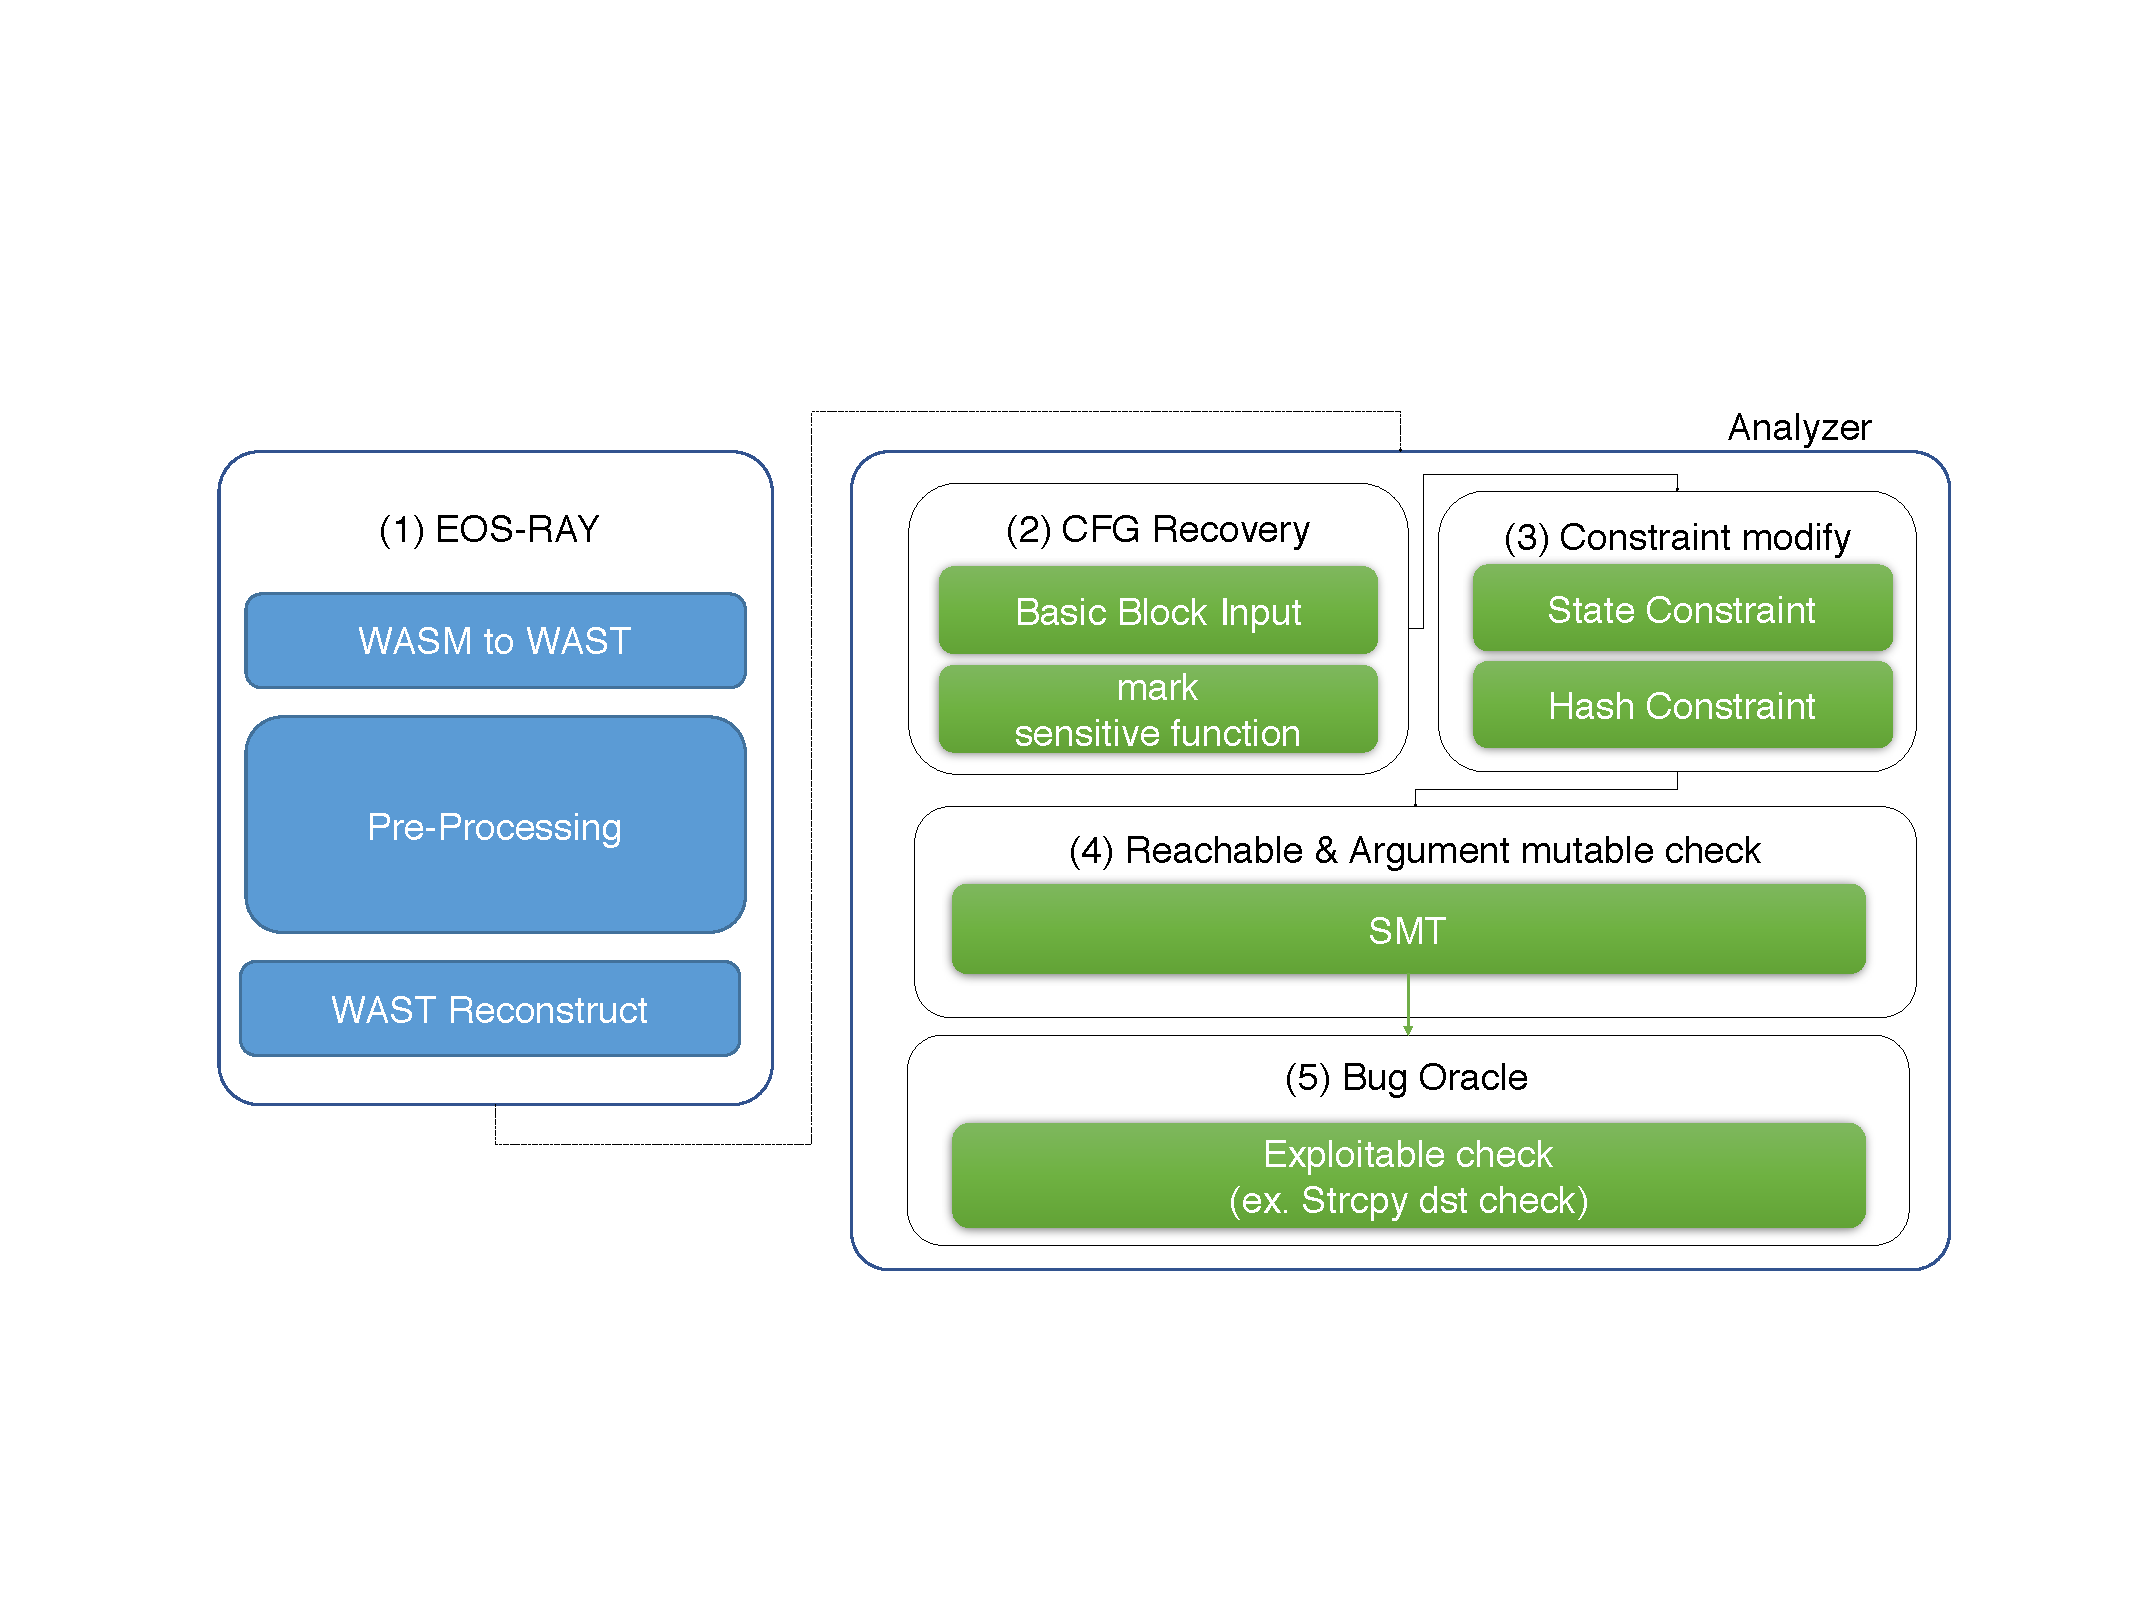
\includegraphics[width=\linewidth]{figures/scalableval.pdf}
  \caption{E-SCV Architecture}

\end{figure} 


%SEED로 사용할 스마트 컨트랙트를 모아야 할 필요가 있다.
%BP Nodeos의 패킷을 분석해 본 결과  "/v1/chain/get\_raw\_code\_and\_abi" 라는 URL 로 producer 의 계정 정보를 보내면 BP nodeos는 자신에게 해당 producer이름으로 등록되 어있는 스마트 컨트랙트와 Abi 를 반환해 준다. 
%eospark 사이트로부터 컨트랙트 1700개 를 수집 할 수 있었으며 관련한 abi도 같이 크롤링 할 수 있었다. 수집된 abi는 컨트랙트의 external method 와 method argument type을 JSON 형식이 아닌 바이너리 형태로 저장하고 있었다.
%json 파일 안에는 "structs" key 를 바탕으로 "name" 과 "fields" value 가 존재하고 "name" value 는 method를 의미하며 "fields" 는 method에 들어갈 type 을 정의하고 있다. 
%"fields"에는 int, account, asset, string 형이 존재하며 이 타입이 맛지 않은 상태로 메소드를 호출 할수 없다. 
%우리는 이러한 external method 들중 action으로 구분되어 실제 이벤트를 실행 할수 있는 함수들 선별하고, 그에 맞는 argument type을 자동으로 파싱하고 값을 대입하여 자동으로 다양한 SEED 컨트랙트의 모든 메소드를 호출 시키도록 구현 하였다. 이렇게 모든 메소드를 호출 시키는 이유는 메소드가 다른 내부 api들을 호출 하는 트리거 포인트가 된다.
\section{Crawling EOS Smart Contract}
We have collected web-assembly smart contracts for use as seed files.
We also do analysis BP Node's packets to collect smart Contracts from producers. we can use  "get\_raw\_code\_and.abi" URL which returns smart contracts and Abi files from producer ID. As a result, we can get not only 2960 smart contracts but also Abi files that are existed as binary types, not JSON formats from the Eos-park web site.
there is various information for calling methods in an ABI file as dictionary styles. 
the Action type includes callable function list, and Structs have arguments types which are consist of Names, Fields. Name field means a Method name, Field field means a type of arguments.
Fields are consist of "int", "account", "asset", "string" and so on. Clients have to call smart-contract methods with correct field types and correct data. So, we need to extract a callable methods name from an Action field and should make correct arguments from struct fields from the struct field automatically. This progress is inevitable for the running smart contract method correctly.

%node 에서 가져온 ABI 파일들은 사람이 읽기에 부적합 하다. 
%우리는 이 바이너리 포멧파일에서 앞서 필요한 method 이름, argument 타입정보등을 가져오기 위해 데이터를 카빙하여 JSON 형태로 변환 해 주었다.
%바이너리 포멧의 ABI 파일의 특징은 아래와 같다.
\section{Regulating binary format ABI to JSON format ABI}
ABI file which is coming from BP Node is not readable format. 
We extracted data which is needed to call smart contract such as method Name, argument types from binary format ABI as reverse-engineering. and We transform this data into JSON file format. 
We analysis the binary format and the pattern is below.
%ABI 바이너리 파일을 hex로 열어보면 특정 규칙이 존재한다.
%ABI파일의 제일 첫 1-byte는 버전 정보에 대한 길이 값을 가지고 있다.
%버정 정보를 알아 오기 위해서는 그 길이 값 만큼 다음 바이트를 읽어야 한다.
%이렇게 한바이트에 길이 값만큼 문자열을 읽어 오는 방식의 패턴화 하고 \textit{ Carving[Target]} 라고 부르도록 하자.
%버전 정보의 이름값 바로 뒤에 1바이트는 structs 에 대한 갯수 값이 들어 있다.
%우리는 앞서 구한 횟수만큼 반복하며 \textit{Carving[StructsName]} 방식을 사용 하여 모든 Structs Name 들을 가져 올수 있다. 각 Structs Name 값은 각각의 Field를 갖게된다. 
%를 위해 \textit{Carving[StructsName]}의 다음 바이트에는 각 "structs" Name 의 Field의 갯수를 저장하고 있다. 우리는 기 Field 의 갯수 값을 읽어 반복문을 돌며 \textit{Carving[StructsField]}를 통하여 필드값들을 저장한다.
%Structs Name 이 끝나고 나면 다음은 Action Name 값이 온다.
%Action Name도 structs 와 마찬 가지로\textit{Carving[ActionName]}을 진행하게 되는데 특이한 점은  Action에 대한 값은 앞에 16byte의 헤더가 붙고 17byte 째때 action Name 의 길이 값이 저장된다. 때문에 16 bytes offset 을 가진뒤 데이터를 읽어오면된다.
%다음은 Table 부분이다. 
%Table section도 Action과 마찬가지로 16byte의 헤더를 가지며, \textit{Carving[TableName]}을 통하여 값을 가져올 수 있다.
%각각의 테이블들은 여러개의 Key name들과 key type들을 가지기 때문에 TableName 바로 다음 바이트에 테이블의 type과 name을 위한 리스트의 갯수가 저장된다. 
%여기서 얻은 리스트의 갯수만큼 반복문을 돌며 \textit{Carving[KeyName]}, \textit{Carving[KeyType]}을 통해 값을 가져올 수 있다. %이후 Key Type 을 위한 name 값이 저장되어 있는데 이 또한 갯수만큼  반복문을 통하여 \textit{Carving[KeyTypeName]}을 통하여 가져 올 수 있다.
%이렇게 얻은 데이터를 가지고 개발자에게 친화적인 개발 당시 JSON형태로 복원 시킬 수 있다. 

ABI binary file has a specific file format. you can analysis using hex-editor. 
The first byte which is in the ABI file has the length of the version string. We can get version string from ABI file reading length byte's size. This method which read specific size for the string is shown repeatedly. and let's called this pattern  \textit{ Carving[Target]}. Right after version information string, there are "structs"'s a number value. We can get all the "struct" names using the \textit {Carving [StructsName]} method by Repeating the number of times previously obtained.
Each "struct" Name value has its own Field.
Because of this, After \textit{Carving[StructsName]} 1 byte has values of numbers which mean Field count. we can get all "field" names using the \textit{Carving[StructsField]} method by repeating the number of times previously obtained. 
After "struct" name comes "action name". 
An "action" name is similar to a "struct". we can get an "action" name with \textit{Carving[ActionName]}, but there is a difference that has a 16-byte header. so after 16-bytes, there is the "Action" name string.
the next format is "table".
A "table" part also has a 16-bytes header, and we can get the "Table" name string using \textit{Carving[TableName]}.
Each table has a number of key names and key types. to express this. tableName format next byte is count value for types, names. With same method before, we can get all "type" value and "name" value using the \textit{Carving[KeyName]} and \textit{Carving[KeyType]} method by repeating the number of times previously obtain number. Next byte is name for "key type" it also could get using \textit{Carving[KeyTypeName]}.



\section{EOSRAY}
%%%%%%%%%%%%%%% 모든 설명은 현재형 %%%%%%%%%%%%%%%%%%%%%%%%%%
% 왜 필요 한지에 대한 설명 (Why)
% 어떠한 방식으로 설계되었는지 설명. (How) 
% 어디에 쓰일 것인지에 대해 설명 (What)
%%%%%%%%%%%%%%%%%%%%%%%%%%%%%%%%%%%%%%%%%%%%%%%%%%%%%%%%%%%%%%%%%%%%
%WASM 파일을 분석하는 프레임워크를 만들기 위해 분석하기 어려운 WASM 바이트 코드의 형태를 분석하기 좋은 WAST 형태로 변형 시키켜야 했고, 이를 위해 EOS SDK에서 제공하는 WASM-DIS 파일을 사용하였다. 
%WASM-DIS파일은 바이트 코드 형태의 WASM파일을 WAST형태로 변형시켜 준다. WAST 파일은 좀더 개발자 친화적인 어셈블리 코드로서 우리는 이 WAST파일을 시작으로 분석툴을 개발 하였다. WAST 파일은 크게 8개지 타입으로 이뤄져 있다.;export, import, type, elem, data, global, function and call instruction.
%항목 타입 들중 function은 메인 코드가 들어 가 있는 항목이다. 이 메인코드는 stack machine 기반으로 처리 하기 좋은, 형태로 되어 있다. E-SCV는 이러한 코드들을 연산 순서 기준으로 스택 구조로 가지고 코드를 에뮬레이팅 하듯 순차적으로 처리를 하며 C언어 형태로 변환한다. 이때 각 분기를 구분하기 위한 label을 추가로 스택에 집어 넣고, label 별로 블럭을 나누어 코드로 표현한다. 이러한 변환을 위해 E-SCV 코드 내에는 웹어셈블리의 172개 instruction을 모두 C언어 형태의 문법으로 재정의 했다. C언어 문법의 형태의 연산자는 Analyzer section의 Symbolic execution에 input값으로 활용된다.  EOSRAY의 중간 산출물은 C언어 형태에 가까운 pseudo code가 되며 이러한 pseudo code를 기준으로 취약점 검증을 수행 할 수 있었다.
We need to change WASM-file to WAST-file which is a more convenient type for analysis. Fortunately, The EOS foundation gave the tools called "wasm-dis" to developers for transforming from wasm-file to wast-file. thus, We also used "wasm-dis" binary file for converting wasm to wast. There are 8-types in web assembly; export, import, type, elem, data, global and function. Among them, main source codes are inside function type, and action-method-functions are being inside elem type. We re-defined all web-assembly instructions, which are 172 instructions, to C-level pseudo-codes so that we can follow control flow from a function of elem to end of that function. The C-level pseudo-codes include various expressions. The various expressions are used to the symbolic execution's input value, and we talk about this Analyzer sections.


\section{Analyzer}
%스마트 컨트랙트의 취약점의 기준은 외부에서 입력된 데이터가 취약한 함수 까지 도달을 하는지를 보는 것이 핵심이다. 실제 취약한 함수가 존재하더라도 사용자에 의해 트리거 될수 없다면 이는 취약한 컨트랙트가 아니다. 이를 자동으로 판단하기 위해 E-SCV는 EOSRAY에서 만들어진 자료구조를 활용하여 취약점을 자동는 알고리즘을 적용하기 좋은 자료구조 형태로 변환한다. 변환된 자료구조는 Symbolic Execution을 통하여 모든 code coverage를 측정하고, 외부에서 입력 가능한 input data를 미지의 변수로 두고 민감한 민감한 함수로 sink 할 때까지 조건식들을 계산하여 외부에서 들어올 수 있는 데이터 인지 아닌지에 대해 판별하게 되며 구체적인 구현은 subsection에서 위 그림과 같은 순서대로 설명 할 것이다.
% 왜 필요 한지에 대한 설명 (Why)
% 어떠한 방식으로 설계되었는지 설명. (How) 
% 어디에 쓰일 것인지에 대해 설명 (What)

The main standard point that decides a bug is that data reachability. Which means that if the sensitive function exists in the function without input data, it is not a bug. thus, E-SCV makes Control-flow-graph(CFG) base on basic block units to the tree data-structure shape. After that, E-SCV mark function's arguments and track the arguments every single step. If the argument reach branch, E-SCV judge reachability using taint analysis. This process is terminated when arguments reach the leaf node or sensitive function. 

\section{CFG recovery}
%control-flow-graph(CFG) recovery는 일반적인 프로그램 자동 분석 시스템에서 자주 사용되는 기법이다.  이렇게 만들어진 각각의 베이직블럭의 자료구조에는 각 블럭에서의 변수값의 변위를 tracking할 수 있도록 저장하고 있고, 각 블럭별 코드에서 사용된 코드들의 연산들을 일괄적으로 관리 하고 있다. 
Control-flow-graph(CFG) recovery is used to automatic analysis for binary programs. It makes we are able to find whole code-coverages. teTher~\cite{krupp2018teether}, which is ethereum audit tool, also uses this method. We adopt the CFG recovery methodology to web assembly smart contracts, and it is base on the basic block tree. E-SCV builds the basic-block-tree with expressions that are used each basic block.


\begin{table}[!t]
\caption{Estimated insecure stmart contracts}
\label{escvTable}
%\begin{center}
\begin{tabular} {ccccccccccc}
\hline\hline
& & send\_dereffered[] & db\_store\_i64[3-5] & db\_update\_i64[\^1][2] & memcpy[2] & strcpy[2] \\
\hline
& $Total API calls$	& 790 	&  	8,059	& 11,620	& 205,033 	& 63	&\\
& $Reachable APIs$	&  117 	&	11		& 7			& 393		& 1		&\\
\hline\hline
\end{tabular}
\begin{tablenotes}
\item Total: 2960 smart-contracts
\item "[num]" means that argv[num] reachability
\item "[\^n]" means that All argument except argv[\^n]
\end{tablenotes}

%\end{center}

\end{table}


\section{Reachability}
%각 Basic Block 단위로 나뉘어진 PATH를 이용해 취약한 함수가 마킹된 블록에 도달이 가능한지 확인하고, 해당 함수가 유저에 의해 조작이 될 수 있음을 확인해야 한다. 
%따라서, 함수가 포함된 블록부터 엔트리 함수까지의 경로에 저장된 Constraint를 Depth First Search(DFS) 알고리즘으로 구한 뒤,
%각 블럭을 순회하는 기준은 Depth first search(DFS) 기준이며, code의 flow가 정의된 취점에 민감한 함수에 도달 할 경우, back-tracing 을 하며 지금까지 거쳐왔던 노드들의 자료구조에 저장된 변수들과 연산자들을 계산하며 빠져나오게 된다.
%satisfiability-modulo-theories(SMT) Solver의 조건에 스택 형태로 삽입 하여 풀이 함으로써 우리가 넣은 어떤 인자에 의해 조작되는지 알 수 있다. 즉, 엔트리 함수, 취약 함수, 인자 번호, 영향을 미치는 입력 값 쌍에 대한 정의를 함으로써 버그 오라클 과정에서 사용될 데이터를 만들어낼 수 있다.
% 엔트리 함수, 취약 함수, 인자번호, 영향을 미치는 입력 값 세트 수식 형태 예시 만들 수 있을듯?
After re-constructing, E-SCV has to mark the function's arguments and track the arguments every single step and make sure reachability to sensitive functions and argument manipulatable via users. Therefore, E-SCV calculates every instruction and data along to constraint-path as Depth First Search(DFS) method. If the code flow can be reached to sensitive functions, E-SCV could solve conditional equations using satisfiability-modulo-theories(SMT) Solver, while back-tracing every basic block with saved variables and expressions but this part is not implemented yet. For now, the Only thing have is input reachability to sensitive functions using taint analysis.


% send_dereffer(), db_update_i64, db_store_i64, memcpy etc... 
\section{Sensitive Functions}
The send\_dereffer() API use EOS-CPU which has to staking EOS coin. So, To reduce unnecessary waste of resources, If the developer wants to use send\_dereffer() APIs, s/he is supposed to set authorization for using its. db\_update\_i64() and db\_store\_i64() are also have to set strict ram-payer for preventing overcharge EOS-RAM which has to purchase by not only attacker but also benign users. This is just the developers mistake. so we evaluated how many smart-contracts that have mistake is being in real EOS-ecosystem using E-SCV.

\section{Limitation and Evaluation}
%이러한 방법론에는 두가지 제한 사하잉 있다. 하나는 상태조건에 따른 함수들의 제한이 있을때이며, 두번째는 두개의 context흐름 서로 유기적으로 연결되어 있을때 이다. 

%예를들면 smart contract에 저장된 데이터를 불러와서 그 값에 의해 취약한 함수가 트리거 되는 케이스이다. 이 경우에는 외부에서 전달되는 값이 직접적으로 취약한 함수로 전달되지 않기 때문에 위 방법으로는 탐지가 되지 않는다.

%두번째는 sensitivie function에 인자가 도달하지만 특정 조건을 만족(컨트랙트에의해 허가된 사용자)하거나 값을 검사하는 로직이 
%pre-condition에 존재하는 경우는 문제가 없는 데이터만 전달 되기 때문에 취약하지 않다. 이러한 검사 로직에 어떠한 것들이 존재하는지 확인하고 condition을 만족하는지를 판단해야만 하지만 아직 그에 따른 기능을 구현하지는 않았고 future work으로 남긴다. 

These methodologies have two limitations. First is that when the smart contract has constrained access with the condition of status. and the second case is that when each context is connected with databases directly. 
The "constrained access" means that If the auditing-APIs that are check parameters exist before sensitive data, there is no bug from here. Even If the external parameter reaches the sensitive-functions. To figure out this problem. we should have check a pre-condition APIs but this solution remains in future works.
The "Each context is connected with databases directly" means that If a function loads the data from the smart contracts database and inserts the data into the sensitive-functions then E-SCV could not get detect reachability to sensitive-functions. because the values don't directly come from the external parameters. 


%우리는 먼저 단순히 외부에서 호출되는 함수에 인자가 실제 sensitive 한 function들의 argument로 전달 되는지만을 파악하였고 결과는 표 \autoref{escvTable}와 같다. 우리는 총 2960개의 스마트 컨트랙트에서 sensitive function을 얼마나 많이 호출하는지를 먼저 단순히 찾아 보았고, 그 갯수는 TotalAPIcalls 이다. 
%하지만 sensitive function들의 모든 argument가 취약한 것은 아니다. 각 함수들은 지정된 argument에 해커의 파라미터가 전달 되는 지에 따라 취약한 함수가 된다. db_update_i64 의 경우에는 1번째 인자 ram_payer가 self로 되어있고 2번째 인자(data)를 외부에서 직접 입력이 가능한 부분을 찾아야한다. self 는 하드 코딩되어 있기 때문에, 직접 그 값을 확인 하지는 못하고, 그 self 값을 tracking 하는 것이 아닌 외부에서 전달 되지 않는 것으로 대체한다. 

First, We do search that the argument is simply passed to the sensitive-functions which the externally called functions. And We simply collect how many patterns are being in a total of 2960 smart contracts. The number of result is written in TotalAPIcalls in \autoref{escvTable}.

However, Not All arguments of function which is pass to sensitive-functions are not vulnerable. Each function becomes vulnerable depending on whether the hacker's parameter is passed to the specified argument. In the case of db\_update\_i64, the first argument ram-payer must set as "self" and the second argument which is data must be coming from the external parameters. However, it is hard to directly check the value is "self". thus, We check that the ram-payer is not coming from the outside instead of the value is set by "self".
%db_store_i64 역시 같은 방식으로 3번째 인자(payer)가 외부에서 들어오지 않고, 5번째 인자 (buffer)가 외부에서 들어오는 함수들에 대해서 검출한다. 
%memcpy의 경우 0번째 인자(dest)와 상관없이 1번쨰 인자(buffer)와 2번째인자 (size)가 외부에서 들어오는 함수들만을 검출하며strcpy 역시 마찬가지이다. 
%EOS-CPU, EOS-NET drain attack에 문제가 되는 send\_dereffer()의 경우에는 일반적으로 smart contract로부터 user-권한의 요청이 없는 한 contract 가 EOS-CPU, EOS-NET을 호출 하므로 send\_dereffer() 함수 이전에 require_auth 가 없는 것을 기준으로 검출하였다. 
In the same way, db\_store\_i64 detects functions from which the third argument (payer) does not come from the outside and the fifth argument (buffer) comes from the outside.
In the case of "memcpy" is that It detects that 1-argument which means buffer is coming from the external parameters.
In case of send\_dereffer() which mention of EOS-CPU and EOS-NET drain attack is detected based on the absence of require\_auth before the function. Because send\_dereffer() API used to use its EOS-CPU and EOS-NET normally.
%우리는 위와 같은 기준으로 도달 여부를 판단하여 \autoref{escvTable}의 reachableAPI 표에 표기한다.
We determined the reachability with these criteria and the result is reachableAPI in table \autoref{escvTable}.


% send_deferred(sender_id, payer.value, serialize.data(), serialize.size(), replace_existing);
% db_update_i64(int32_t iterator, account_name payer, const void* data, uint32_t len)
% apply_context::db_store_i64( uint64_t code, uint64_t scope, uint64_t table, const account_name& payer, uint64_t id, const char* buffer, size_t buffer_size ) 


